%% bare_jrnl.tex
%% V1.4b
%% 2015/08/26
%% by Michael Shell
%% see http://www.michaelshell.org/
%% for current contact information.
%%
%% This is a skeleton file demonstrating the use of IEEEtran.cls
%% (requires IEEEtran.cls version 1.8b or later) with an IEEE
%% journal paper.
%%
%% Support sites:
%% http://www.michaelshell.org/tex/ieeetran/
%% http://www.ctan.org/pkg/ieeetran
%% and
%% http://www.ieee.org/


\documentclass[journal]{IEEEtran}


\usepackage{times}
\usepackage{epsfig}
\usepackage{graphicx}
\graphicspath{{images/}}
\usepackage[justification=centering]{caption}
\usepackage{subfigure}
\usepackage{float}
\usepackage{amsmath}
\usepackage{amssymb}
\usepackage{multirow}
\usepackage{cite}
\usepackage{bm}
\usepackage{hyperref}
\makeatletter
\newcommand{\rmnum}[1]{\romannumeral #1}
\newcommand{\Rmnum}[1]{\expandafter\@slowromancap\romannumeral #1@}
\makeatother



% correct bad hyphenation here
\hyphenation{op-tical net-works semi-conduc-tor}


\begin{document}

\title{Small Target Detection in Infrared Video \\Based on Spatio-temporal Tensor Model}
%
%
% author names and IEEE memberships
% note positions of commas and nonbreaking spaces ( ~ ) LaTeX will not break
% a structure at a ~ so this keeps an author's name from being broken across
% two lines.
% use \thanks{} to gain access to the first footnote area
% a separate \thanks must be used for each paragraph as LaTeX2e's \thanks
% was not built to handle multiple paragraphs
%

\author{Hongkang~Liu,~Lei~Zhang,~\IEEEmembership{Fellow,~IEEE}
        and~Hua~Huang,~\IEEEmembership{Fellow,~IEEE}% <-this % stops a space
\thanks{M. Shell was with the Department
of Electrical and Computer Engineering, Georgia Institute of Technology, Atlanta,
GA, 30332 USA e-mail: (see http://www.michaelshell.org/contact.html).}% <-this % stops a space
\thanks{J. Doe and J. Doe are with Anonymous University.}% <-this % stops a space
\thanks{Manuscript received April 19, 2005; revised August 26, 2015.}}

% note the % following the last \IEEEmembership and also \thanks - 
% these prevent an unwanted space from occurring between the last author name
% and the end of the author line. i.e., if you had this:
% 
% \author{....lastname \thanks{...} \thanks{...} }
%                     ^------------^------------^----Do not want these spaces!
%
% a space would be appended to the last name and could cause every name on that
% line to be shifted left slightly. This is one of those "LaTeX things". For
% instance, "\textbf{A} \textbf{B}" will typeset as "A B" not "AB". To get
% "AB" then you have to do: "\textbf{A}\textbf{B}"
% \thanks is no different in this regard, so shield the last } of each \thanks
% that ends a line with a % and do not let a space in before the next \thanks.
% Spaces after \IEEEmembership other than the last one are OK (and needed) as
% you are supposed to have spaces between the names. For what it is worth,
% this is a minor point as most people would not even notice if the said evil
% space somehow managed to creep in.



% The paper headers
\markboth{Journal of IEEE Transactions on Geoscience and Remote Sensing,~Vol.~14, No.~8, August~2018}%
{Shell \MakeLowercase{\textit{et al.}}: Bare Demo of IEEEtran.cls for IEEE Journals}
% The only time the second header will appear is for the odd numbered pages
% after the title page when using the twoside option.
% 
% *** Note that you probably will NOT want to include the author's ***
% *** name in the headers of peer review papers.                   ***
% You can use \ifCLASSOPTIONpeerreview for conditional compilation here if
% you desire.




% If you want to put a publisher's ID mark on the page you can do it like
% this:
%\IEEEpubid{0000--0000/00\$00.00~\copyright~2015 IEEE}
% Remember, if you use this you must call \IEEEpubidadjcol in the second
% column for its text to clear the IEEEpubid mark.



% use for special paper notices
%\IEEEspecialpapernotice{(Invited Paper)}




% make the title area
\maketitle

% As a general rule, do not put math, special symbols or citations
% in the abstract or keywords.
\begin{abstract}
Existing methods for infrared small target detection are not effective under highly complex backgrounds condition. It is mainly caused by: (1) the interference of strong edges and other similar-target components. (2) not making full use of the context information of background and target in spatio-temporal domain. Inspired by this, we form a spatio-temporal cube with current image patch and adjacent image patches in spatio-temporal adjacent domain, then we establish a spatio-temporal tensor model for small target detection. According to the sparse prior of target and the local correlation of background, the target-background separation problem is transformed into a low rank-sparse tensor decomposition problem. The target image is reconstructed from the sparse tensor obtained after tensor decomposition. The experiment results show that our method could make full use of the context information in spatio-temporal domain in infrared video. Compared with other methods, our method has better detection performance in several videos with highly complex backgrounds.
\end{abstract}

% Note that keywords are not normally used for peerreview papers.
\begin{IEEEkeywords}
Infrared video, small target detection, spatio-temporal tensor model, tensor decomposition.
\end{IEEEkeywords}


%Intruction
%
%

\section{Introduction}

\IEEEPARstart{A}{t} present, infrared target detection technology has been widely used in missile tracking, precision guidance, early warning, maritime surveillance, ground monitoring\cite{luo2015space,dawson2010space,li2014infrared}, etc. Compared with ordinary detection tasks, lacking of sufficient information to determine the target is the main challenge of small target detection in infrared image. Due to the long infrared imaging distance, the size of small targets in infrared image is very small, generally ranging from $2\times2$ to $9\times9$ pixels\cite{wang2017infrared}. And in the case of long imaging distance, the small targets in infrared image has no fixed shape and stable texture features. In addition, the infrared radiation of targets is heavily attenuated after long-distance propagation, which results in a low signal-to-noise ratio (SNR) for small infrared targets\cite{li2016novel}. When there are complex background clutter and noise, small targets with low signal-to-clutter ratio (SCR) are usually buried in background. Therefore, the detection of small targets under a complex infrared background is remaining a problem that is full of difficulty and challenges.

Compared with visible image, infrared image look simpler. However, infrared image lacks color information and texture information, and has poor image quality usually, which cause great difficulty in the process of small target detection.The lack of color information will result in fewer features for distinguishing between target and background. The lack of texture information and shape information means that the target cannot be distinguished based on the feature learning of the small target. Therefore, utilizing not only the relationship between small target and background, but also the motion characteristics of target is an important way to detect infrared small targets.

The small target detection methods in infrared image are mainly divided into two categories: single-frame image detection methods which use spatial domain information and spatio-temporal detection methods which utilize inter-frame temporal domain information and intra-frame spatial domain information\cite{li2016novel}. There are often some special backgrounds, such as man-made objects and cloud patch, which will interfere with the target detection task, and the imaging resolution and SCR of small target are smaller than expected. Therefore, it is impossible to identify target by using only the information in spatial domain, and the small target on a single image is invisible in perception. According to above analysis, it is extremely important to make full use of the context information of small target in the temporal domain. The current spatio-temporal detection methods usually calculate the local contrast of spatial domain and temporal domain separately, and combines them to detect the small target. However only calculating of local contrast will not identify true small targets in the case of complex noise or the motion of background, resulting in excessive false alarms and missing alarms. In order to make full use of the effective information of temporal domain and spatial domain, and to avoid the influence of noise when detecting, we propose a method for small target detection based on spatio-temporal image patch tensor decomposition. The main contribution of this paper is as follows: The proposed spatio-temporal tensor model considers the local correlation of the background image patch in spatial and temporal neighborhood domain, so it will suppress the background clutter better. And our method not only reflects the spatial significance of target, but also make full use of the motion characteristics of small target, utilizing the sparse characteristics of small target in spatio-temporal neighborhood domain.

The remaining chapters of this paper are organized as follows: We introduce the related researches of infrared small target detection in section \Rmnum{2}; And in section \Rmnum{3} we propose the spatio-temporal tensor model and the method for detecting infrared small targets via spatio-temporal image patch tensor model in detail; In section \Rmnum{4},we verify the effectiveness of the proposed method via a large number of experiments; In section \Rmnum{5}, we give the conclusions and prospects for future.

%Related work
%
%
\section{Related Work}
At present, the methods proposed for detecting small moving targets in infrared video can roughly classified into two categories. The first major category is mainly performing target detection on a single image. Another category detect small targets utilizing multiple images from a infrared video.

\subsection{Detection Methods Based on Single Image}
The methods for target detection via single image frame are further divided into two types, which are based on the following two assumptions. The first type of methods are based on a classic assumption that background changes slowly in infrared images and high correlations exist between adjacent pixels. Another type of methods based on single image frame utilize the non-local self-correlation between background pathes in infrared image. It is usually assumed that all background image patches in infrared image are from a low-rank subspace or a mixed set composed with multiple low-rank subspaces\cite{liu2013robust}.

Based on the first hypothesis, some classical methods based on image filtering are proposed, such as two-dimensional minimum mean square error filtering\cite{hadhoud1988two}, maximum median and maximum mean filtering\cite{deshpande1999max}, transform domain methods \cite{davidson2002wavelet,peng2004dim} and so on. This type of methods enhance small targets by calculating the difference between original image and predicted background. Other methods have been proposed with extensive research in human visual system, such as Laplacian Gaussian (LoG) filter based methods\cite{kim2009small}, Gaussian difference (DoG)\cite{wang2012infrared} and second-order directional derivatives\cite{qi2013robust}. Although this type of methods can reduce the influence of edge compared with traditional method, it can not suppress the clutter and strong edges in complex background, resulting in many false alarms. Meanwhile, there is usually a large difference between infrared small target and surrounding background, based on which some methods based on local contrast are proposed, such as local contrast measurement method (LCM)\cite{chen2014local}, improved local contrast measurement (ILCM)\cite{han2014robust}, image block based multi-scale contrast measurement (MPCM)\cite{wei2016multiscale} and so on. Similarly, other methods such as local difference measurement (LDM)\cite{deng2017entropy}, local significance map (LSM)\cite{chen2016efficient} and weighted local difference measure (WLDM)\cite{deng2016small} have been proposed in succession. This traditional type of methods can suppress background and enhance small targets, but a large amount of noise and clutters are also enhanced in the case of complex background, and are considered as small targets by mistake. So the false-alarm rate of these methods are usually high and the practicability is reduced also.

Based on the second hypothesis, small target detection in infrared image can be transformed into a low-rank matrix recovery problem. Gao\cite{gao2013infrared} et al. proposed to convert the traditional infrared image model into a new infrared image patch model, and considered that background has low rank characteristics and the small targets are sparse relative to the whole image. Therefore target could be separeated from background via recovering low-rank and sparse matrices. However, the method still has insufficient effect when processing strong edges and clutters, so RIPT\cite{dai2017reweighted} extract prior features via local structure information , and then suppress edges with local structure weight in the process of small target detection. However in the case of complex background, the image patches may come from multiple low-rank subspaces, so Wang\cite{wang2017infrared} et al. use a multiple-subspace learning strategy to better suppress background, whih can effectively reduce false alarm rate. The above methods are based on robust principle component analysis (RPCA) to achieve small target detection. But, due to the existence of many clutters in background in single image, such as cloud patches in sky and fixed heat objects on ground, the detection of true targets will be interfered seriously. The information of single image is not sufficient to identify small targets, so it is necessary to take temporal information into account including motion information of target and context information of background.

\subsection{Detection Methods Based on Multiple Images}
The second major mathods for infrared small targets detection are mainly based on multiple images from infrared video. These methods make full use of information in spatial domain ton suppress background clutters and utilize motion characteristics of targets to highlight small targets. Therefore better detection results could got. Silverman and Caefer et al. utilized temporal information for small target detection, and proposed Recursive Variance Filter (TVF)\cite{silverman1998temporal} and Damped Sinusoid Filters (TTF)\cite{caefer1998temporal}. But the difference of target and moving background can not be reflected according to temporal information only. For example, moving cloud may be detected as true target. And then Deng et al.\cite{deng2016infrared} proposed a spatial-temporal local contrast filter for infrared small target detection, but the calculation of local contrast via pixels is easily affected by noise. Gao et al. proposed TVPCF\cite{gao2017tvpcf} which combines multi-scale local contrast based on patches with temporal filter to obtain better detection results. Li et al.\cite{li2016novel} proposed a new way to calculate local contrast. Image patches in spatio-temporal neighborhood of current image patch are used to reconstruct a new image patch. The residual of current image patch and reconstructed image patch is defined as local contrast. Although this method can suppress clutters and single pixel noise, the reconstruction process is extremely sensitive ton noise. Therefore many targets will be missed under high noise.

\begin{figure*}[htb]
  \centering
  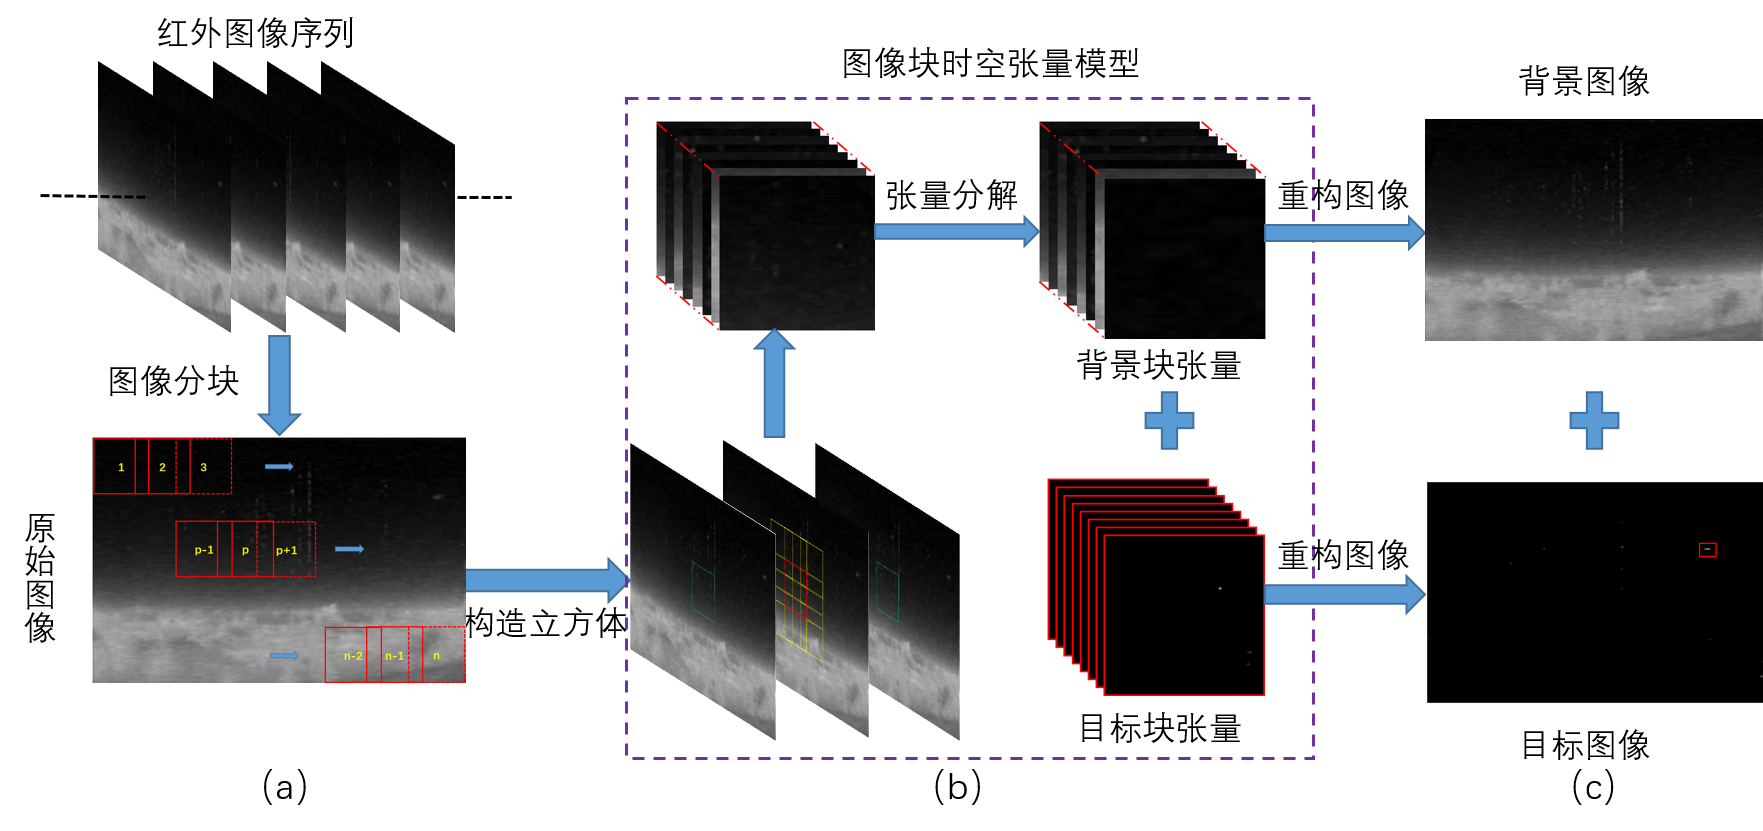
\includegraphics[width=0.9\textwidth]{flow_chart.png}
  \caption{The flow chart of small target detection based on spatio-temporal tensor model}
  \label{fig:flow_chart}
\end{figure*}


\section{Construction and Decomposition of Spatio-temporal Tensor Model}
Due to the traditional imaging mechanism, there is usually a strong correlation between background image patches in spatial adjacent domain. And background moves slowly compared with target, so background image patches also have strong correlations in temporal adjacent domain. Then, single image is segmented into image patches by sliding window, and an image patch cube is formed by current patch and patches from the spatial and temporal adjacent domain of current patch. The image patch cube is viewed as a spatio-temporal tensor. In the spatio-temporal tensor, background tensor is low-rank and target tensor is sparse. Therefore the target tensor can be decomposed from original tensor, then target patch is separated from original patch. The specific construction method and decomposition process of spatio-temporal tensor model will be described in detail in this section.


\subsection{Construction of spatio-temporal tensor model}
In order to make more use of the relevant information between backgrounds in infrared frames, we propose a new target and background separation model called the spatio-temporal tensor model in this section. Usually, the infrared image model is defined as follows for infrared small target detection similar to\cite{gu2010kernel}:
\begin{equation}
  f_D(x,y)=f_T(x,y)+f_B(x,y)+f_N(x,y)
  \label{eq:image_model}
\end{equation}
where $f_D,f_T,f_B,f_N \text{ and } (x,y)$ corresponds to the original infrared image, the target image, the background image, the noise image and the position coordinates of each pixel respectively.

Figure 1(a) shows the construction process of spatio-temporal image patch tensor. Firstly, the original image is divided into several image patches via sliding window from top to bottom and left to right. For each image patch, $m_t$ image patches in temporal adjacent domain and $m_s$ image patches in spatial adjacent domian (including itself) are collected to form a spatio-temporal cube. The spatio-temporal cube is also viewed as a tensor called spatio-temporal image patch tensor. Spatial image patch tensor and temporal image patch tensor are constructed 
as shown in figure 1(b):
\begin{equation}
  \begin{split}
    \bm{D}_t = \bm{B}_t + \bm{T}_t + \bm{N}_t \\
    \bm{D}_s = \bm{B}_s + \bm{T}_s + \bm{N}_s
  \end{split}
\end{equation}
where $\bm{D}_t,\bm{B}_t,\bm{T}_t,\bm{N}_t \in R^{{I}\times{J}\times{m_t}}$ are the tensors composed with original image patches, background image patches, target image patches and noise image patches from spatial adjacent domain separately. Moreover, $\bm{D}_s,\bm{B}_s,\bm{T}_s,\bm{N}_s \in R^{{I}\times{J}\times{m_s}}$ are are the tensors composed with original image patches, background image patches, target image patches and noise image patches from temporal adjacent domain separately. $I\text{ and }J$ correspond to the height and width of image patch, respectively, depending on the size of sliding window. Then, the context information in spatial and temporal adjacent domain could be utilized by us at the same time, so the following tensor model can be formed by combining the spatial and temporal tensor mentioned above:
\begin{equation}
  \bm{D}=\bm{B}+\bm{T}+\bm{N}
\end{equation}
where $\bm{D},\bm{B},\bm{T},\bm{N} \in R^{{I}\times{J}\times{(m_t+m_s)}}$.

The context information of background in temporal domain and spatial domain can be utilized simultaneously according to the above model. Nextly, we will analyze the characteristics of each component in spatio-temporal image patch tensor in detail. And we will give the solution algorithm for our spatio-temporal tensor model on the basis of classical low-rank tensor recovery algorithm to detect small targets in infrared video.

\subsection{Background image patch tensor $\mathbf{B}$ }
In general, the movement of background is slow relative to small targets, so there are high correlations between background image patches in temporal neighborhood. Moreover, the imageing principium in infrared video causes that the image patches are also correlated within spatial local neighborhood. At present, the most advanced IPI\cite{gao2013infrared} model adopts the non-local correlation of background image patches, but we adopt the local correlation of them. The reason why we adopt the local correlation of background image patches is that the local correlation is stronger than non-local.

In order to compare with traditional IPI model for convenience, our spatio-temporal tensor model selects several background image patches in spatio-temporal adjacent domain, and the IPI model randomly selects same number of background image patches of non-local regions. Then we transform the spatio-temporal tensor into a mode-1 unfold matrix. And the singular values are calculated of the matrixs formed by two models. It can be seen from the first and second rows of figure(2) that the singular valuse of spatio-temporal tensor which utilizes the local correlation of background image patches decrease faster. It proves that the background tensor in our model has better low-rank characteristics, so it can be ensured that there will be fewer background components (clutters) in targetb tensor during the decomposition process.
\begin{figure}[H]
  \centering
  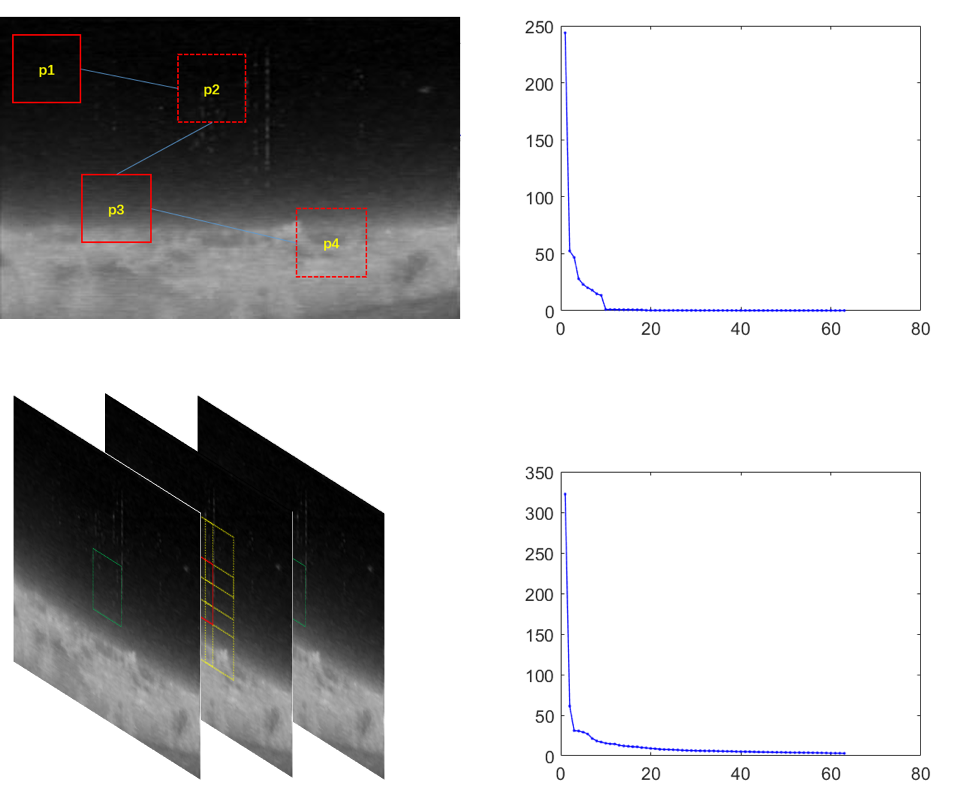
\includegraphics[width=0.5\textwidth]{singular.png}
  \caption{First row: singular value curve for non-local correlation;\\Second row:singular value curve for local correlation}
  \label{singular}
\end{figure}

From the above analysis, the background tensor is low-rank:
\begin{equation}
  rank(\bm{B}) \leq r
\end{equation}
where $r$ is a low-rank constant constraint corresponding to background tensor. Usually $r$ is bigger in complex background than uniform background.


\subsection{Target Image Patch Tensor $\mathbf{T}$}
In actual application scenario, due to the infrared imaging characteristics, there is no obvious texture information and color information of small targets in infrared video. And the sizes of different targets also vary within a certain range. Moreover, the brightness of infrared small target is also different in different scenes. But infrared small targets are always small in size because of that imaging distance is far. So if small target appears in spatio-temporal patch cube, the volume occupied by small target is great smaller compared with the volume of entire spatio-temporal patch cube. Specifically expressed as follows:
\begin{equation}
  V(\bm{T}) \ll V(\bm{D})
\end{equation}
Therefore, the target image patch tensor is a sparse tensor actually, and it satisfies:
\begin{equation}
  \left \| \bm{T} \right \|_0 \leq k
\end{equation}
where $k$ is a small constant that can be visually regarded as the volume corresponding to target, which is determined by the size of the target and the number of times that targets appear in the spatio-temporal patch cube.




\section{Conclusion}
The conclusion goes here.





% if have a single appendix:
%\appendix[Proof of the Zonklar Equations]
% or
%\appendix  % for no appendix heading
% do not use \section anymore after \appendix, only \section*
% is possibly needed

% use appendices with more than one appendix
% then use \section to start each appendix
% you must declare a \section before using any
% \subsection or using \label (\appendices by itself
% starts a section numbered zero.)
%


\appendices
\section{Proof of the First Zonklar Equation}
Appendix one text goes here.

% you can choose not to have a title for an appendix
% if you want by leaving the argument blank
\section{}
Appendix two text goes here.


% use section* for acknowledgment
\section*{Acknowledgment}


The authors would like to thank...


% Can use something like this to put references on a page
% by themselves when using endfloat and the captionsoff option.
\ifCLASSOPTIONcaptionsoff
  \newpage
\fi



% trigger a \newpage just before the given reference
% number - used to balance the columns on the last page
% adjust value as needed - may need to be readjusted if
% the document is modified later
%\IEEEtriggeratref{8}
% The "triggered" command can be changed if desired:
%\IEEEtriggercmd{\enlargethispage{-5in}}

% references section

% can use a bibliography generated by BibTeX as a .bbl file
% BibTeX documentation can be easily obtained at:
% http://mirror.ctan.org/biblio/bibtex/contrib/doc/
% The IEEEtran BibTeX style support page is at:
% http://www.michaelshell.org/tex/ieeetran/bibtex/
%\bibliographystyle{IEEEtran}
% argument is your BibTeX string definitions and bibliography database(s)
%\bibliography{IEEEabrv,../bib/paper}
%
% <OR> manually copy in the resultant .bbl file
% set second argument of \begin to the number of references
% (used to reserve space for the reference number labels box)
\bibliographystyle{IEEEtran}
\bibliography{ref}
% biography section
% 
% If you have an EPS/PDF photo (graphicx package needed) extra braces are
% needed around the contents of the optional argument to biography to prevent
% the LaTeX parser from getting confused when it sees the complicated
% \includegraphics command within an optional argument. (You could create
% your own custom macro containing the \includegraphics command to make things
% simpler here.)
%\begin{IEEEbiography}[{\includegraphics[width=1in,height=1.25in,clip,keepaspectratio]{mshell}}]{Michael Shell}
% or if you just want to reserve a space for a photo:

\begin{IEEEbiography}{Michael Shell}
Biography text here.
\end{IEEEbiography}

% if you will not have a photo at all:
\begin{IEEEbiographynophoto}{John Doe}
Biography text here.
\end{IEEEbiographynophoto}

% insert where needed to balance the two columns on the last page with
% biographies
%\newpage

\begin{IEEEbiographynophoto}{Jane Doe}
Biography text here.
\end{IEEEbiographynophoto}

% You can push biographies down or up by placing
% a \vfill before or after them. The appropriate
% use of \vfill depends on what kind of text is
% on the last page and whether or not the columns
% are being equalized.

%\vfill

% Can be used to pull up biographies so that the bottom of the last one
% is flush with the other column.
%\enlargethispage{-5in}



% that's all folks
\end{document}


